\documentclass[conference]{IEEEtran}
\IEEEoverridecommandlockouts
% The preceding line is only needed to identify funding in the first footnote. If that is unneeded, please comment it out.
\usepackage{cite}
\usepackage{amsmath,amssymb,amsfonts}
\usepackage{algorithmic}
\usepackage{graphicx}
\usepackage{textcomp}
\usepackage{xcolor}
\def\BibTeX{{\rm B\kern-.05em{\sc i\kern-.025em b}\kern-.08em
    T\kern-.1667em\lower.7ex\hbox{E}\kern-.125emX}}
\begin{document}

\title{Decentralized Autonomous Rovers\\
{\footnotesize \textsuperscript{*}Freedom Rover Units}
\thanks{}
}

\author{\IEEEauthorblockN{1\textsuperscript{st} Jordy A. Larrea Rodriguez}
\IEEEauthorblockA{\textit{Department of Electrical and Computer Engineering} \\
\textit{University of Utah}\\
Salt Lake City, USA \\
Jordy.larrearodriguez@gmail.com}
\and
\IEEEauthorblockN{2\textsuperscript{nd}  Brittney L. Morales}
\IEEEauthorblockA{\textit{Department of Electrical and Computer Engineering} \\
\textit{University of Utah}\\
Salt Lake City, USA \\
brittneymrls@gmail.com}
\and
\IEEEauthorblockN{3\textsuperscript{rd} Misael Nava}
\IEEEauthorblockA{\textit{Department of Electrical and Computer Engineering} \\
\textit{University of Utah}\\
Salt Lake City, USA \\
misaelnava812@gmail.com}
}

\maketitle

\begin{abstract}
The state of the art in autonomous swarms employs a decentralized model consisting of multi-agent networks. These multi-agent systems hold the potential to adapt to new environments and optimize individual performance to specific tasks without having to deal with global systems prone to single points of failure. Our team's focus lies therein in developing a decentralized multi-agent system. The decentralized multi-agent system will incorporate three to five two-wheel drive rovers interfaced through the Robot Operating System (ROS) by raspberry pi 4 companion computers for edge-computing specifications. A central system is still beneficial for the assignment of global objectives; thus, our proposed decentralized system will employ a central bay station to communicate objectives for the agents to complete (carefully designed demos). LiDAR, simple infrared sensors, and low-resolution cameras will be procured to facilitate real-time (RT) decision-making by the agent(s) in response to the environment. Our development stack will leverage ROS for project management, simulation capabilities, navigation libraries, and native server-client model in robotics applications. The rovers AI will incorporate simultaneous localization and mapping (SLAM) techniques for RT positioning based on a priori grid or map; thus, facilitating navigation through improved state space mapping. Decentralized swarms allow for a set of agents to act as more than distributed actuators: i.e., more like your white blood cells rather than your limb as observed by central systems. Furthermore, drone Swarms hold the potential to gather large quantities of data for monitoring and area mapping that would otherwise prove too costly to collect, and can greatly simplify and reduce manpower in search-and-rescue, disaster recovery, or security scenarios. Swarms essentially hold the capability to replace humans in potentially dangerous and normally costly tasks.
\end{abstract}

\begin{IEEEkeywords}
Decentralized Communication, Swarm Communication, Multi-agent, ROS, Gazebo
\end{IEEEkeywords}

\section{Introduction}
\begin{figure}
	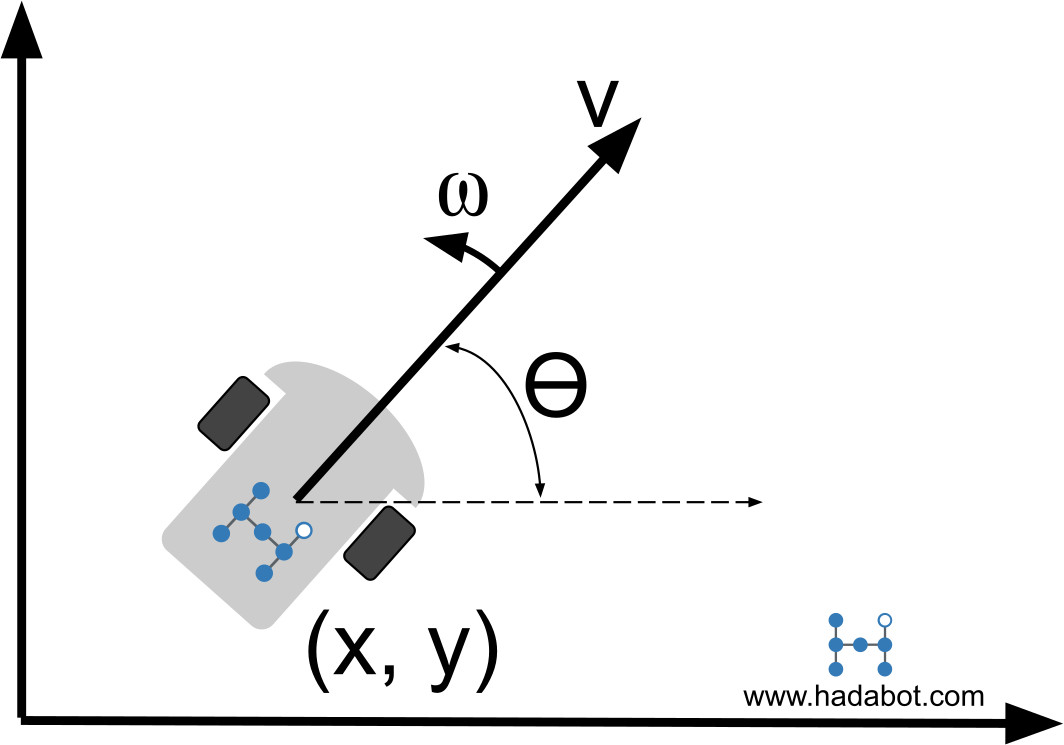
\includegraphics[width=\linewidth]{hadabot_unicycle_diagram_01.jpg}
	\caption{Graphical representation of 2D robot pose information standard to 2 wheel robots \cite{RN109}.}
\end{figure}
As all forms infrastructure continue to evolve and grow in complexity, the pressing need for technology that can function beyond natural human capabilities. Consider industrial accidents, natural disasters, and other catastrophic accidents. Increasing global human population densities risk exacerbated potential fatalities and overwhelmed local services \cite{RN94, RN100, RN104, RN106}. Robots could prove versatile in situations that require human involvement due to the mass-manufacturable nature of cyber-physical systems, advancements to AI, and the negated risk to live human agents. Drones unlike their human counterparts do not need to meet biological requirements for sustained action; thus, drones can be deployed for a substantial amount of time without rest, can navigate spaces hazardous to humans, can loco-mote via flight, can reach high speeds, can inexpensively monitor expansive industrial or rural areas, and can gather large amounts of data fast and cost effectively \cite{RN101}. In order for drone swarms to reach the level of versatility described above, every agent must make its own decisions in response to the environment and global criteria/task assignments in a collaborative manner with other agents (CITE Basically Everybody). These so called multi-agent systems (MAS) eliminate single points of failures and can complete tasks collaboratively and independently of other agents. Like divide and conquer techniques in modern software solutions, MAS systems can delegate and work together to complete a task without central nodes bottle-necking task completion or MAS response to dynamic environments \cite{RN100}. Thus, our motivation to design and develop a MAS comes from the novel and useful applications of decentralized swarms. Currently, ROS and Gazebo have been used widely for simulation in robotics and MAS projects. ROS itself was born due to an inherent need for dynamic and adaptive control from task-specific industrial robots and to decrease the development time of robotics projects. ROS incorporates a server-client model where each ‘robot’ running a ROS program is a node that can ‘subscribe’ or listen to certain topics where messaging can then occur. Furthermore, packages and tool-boxes that ship with or are compatible with ROS incorporate path-planning techniques, search and navigation, mapping techniques, control theory, and automation algorithms. MAS projects hold the disadvantage of long debugging times and a necessity for hardware and software to function seamlessly. Three-dimensional simulation software like Gazebo allow for reconstruction of environments and deployment of agents running on experimental software \cite{RN104}. Our team intends on simulating, testing, debugging, and validating our automated agents via Gazebo before deploying them in the real world. The aforementioned approach is recommended both in literature and by industry experts that we spoke with. Computers meant to run complex operating systems like the raspberry pi are inadequate to handle RT control of motors, actuators, and sensors (poor interfacing/port options). Thus, our rovers will incorporate a micro-controller unit (MCU) to run proportional, integral and derivative (PID) control to meet state spaces communicated by a ‘companion computer’ such as a raspberry pi. The rovers will incorporate edge-computing to run their ROS programs on the Raspberry pi, allowing for complex AI algorithms to run within close proximity to the micro-controller: i.e., allowing the MCU to act as the peripheral nervous system of the rover, and the raspberry pi as the brain of the rover. Edge-computing places AI, cloud computing, or data driven models closer to the agent for improved performance and native high level computation. Our approach, schedule, and planned system demonstrations are highlighted in the sections below.

\section{Background} 
\begin{figure}
	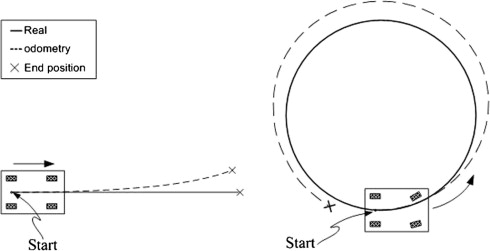
\includegraphics[width=\linewidth]{odometry_error.jpg}
	\caption{Graphical representation of basic odometry error as a robot follows a reference trajectory \cite{RN206}.}
\end{figure}
A plethora of elements must come together to successfully deploy a swarm of decentralized agents. Our system requires a working knowledge in both the physical and abstract. The agents are subject to their physical characteristics: i.e., their circuitry, power consumption, mechanical components, sensors, processing power, and geometry to navigate and respond to an environment. The complexity that drives cyber-physical systems is what largely makes robotics difficult. An agent must be able to function perfectly in a world with a continuous state space. Today, researchers are seeing a high degree of success with robots that incorporate mathematical and data driven modeling that leverages the superior computational capabilities of modern processors to solve complex continuous problems in robotics. 

\subsection{The Odometry Problem and SLAM}Normally, robots use a wide range of sensors to inform themselves about the surrounding environment. Our agents, for example, rely on a 6 axis inertial measurement unit (IMU) and rotatory encoders to produce an \{x,y\} pose (with angle $\theta$) at every time step by considering physical properties and mechanics. Where a pose is simply a state relative to some other state in a previous time step. However, a frequent problem with using rudimentary techniques solely for odometry is that error propagated at each time step due to environmental conditions, sensor specifications, and rounding error can deviate a naive agent during navigation. The problem persists even with the use of a known map and highly accurate sensors. Consider how a human might traverse a city by using a map. The human could ensure their own position by simply pondering their place in respect to features of the map like buildings, intersections, or street signs. Even if the human absent mindlessly navigated the city, they could triangulate their 'pose' by simply calculating their positions based on observations (such as the coffee shop across the street). For an agent, SLAM leverages known knowledge of poses at past time steps and emissions or observations (sensor readings) made as the agent accumulates error through basic odometry to calculate probabilities of where the agent can be in space. Any number of sensors that detect 'emissions' from the environment can be used for SLAM; however, 2D lidar and cameras are regularly used for the high degree of precision awarded. Agents are capable of both learning a new environment and updating a known map with SLAM; thus, justifying our deployment of SLAM to improve the navigation capabilities of each agent.

\section{Scope of Project and Design}The scope/goal of the project is to create a small group(our swarm) of semi-decentralized rovers that achieve a common goal. Our swarms will consist of an aim of 3+ rovers which although does not constitute an ideal amount for a swarm, however this will be enough for a proof of concept for the future that will use a larger group of individuals. As for the common goal, the team of robots should be able to work together to put on a little synchronized dance performance or to push a block from point A to another point in space. While the concept of these rovers being decentralized means that they are able to act independently with assistance from a central leader. This now leads into the question of how these autonomous rovers are going to be made and how they will be aware of their environment.
There are multiple ways we can get the rovers to perceive their surroundings, in the case of the project there are three options. One option is to use a 2D Light Detection and Ranging (lidar) sensor. The lidar will give the robot an image of the objects currently around it and the distance from the unit itself. With the implementation of lidar it will open up the avenue to accurately use SLAM(Simultaneous Localization and Mapping). For the actual build of the rovers the plan is to use a premade chassis for the outer shell of the robot. It will also use two stepper motors and a caster wheel to enable movement. As for powering/controlling the system, it will use a custom PCB power module for powering the different components with another custom PCB motor driver to control the stepper motors.

\section{Methods and Planning}


\subsection{Initial Timeline and Project Tasks}\label{AA}
Most milestones will be collaborative, meaning they are not going to be directly assigned to people on the team. The only exception is the first milestone where the team members that still do not have a good understanding of ROS will work on becoming familiar with it. However, mini-milestones will be assigned as the team gets to them. An example of this is when it comes to testing parts each person will choose which part they will test. The same will go with coding aspects of the project and these assignments will be documented to keep track of who has worked on what. Here is the initial timeline for the project broken down into individual tasks:
\begin{itemize}
	\item May: Assemble Rover/PCB/Get Better understanding of ROS
	\begin{itemize}
		\item Main goal is to make the custom PCB for power module and motor drivers
		\item Buy parts: Motor, Chassis, LiPo Battery, development boards, environment sensing parts
		\item Test PCB and parts to make sure they are functional and understand how to interface with them
		\item Become familiar enough with tools to begin code development
	\end{itemize}
	\item June: Setup ROS/Code Framework
	\begin{itemize}
		\item Use ROS to create initial code for the multi-agent server to assist Rovers
		\item Also use ROS to manipulate and control motors to allow Rover to move
		\item Begin interfacing with sensors and other components
	\end{itemize}
	\item July: Setup ability to see environment
	\begin{itemize}
		\item Setup Lidar/Computer Vision
		\item Get Rovers to build map of their environment SLAM
		\item Ensure rovers can move through environment without colliding
	\end{itemize}
	\item August: Get Rover to move in consistent manner and Implement Agent AI
	\begin{itemize}
		\item Finish up main part of Rover framework
		\item Get the Rovers to move in a set pattern
		\item Work on the AI for rovers
	\end{itemize}
	\item September: Setup central server/Test Communication
	\begin{itemize}
		\item Finish creating ROS multi-agen server
		\item Get the server to communicate with Rovers
		\item Test reaction time between server and Rovers
	\end{itemize}
	\item October: Rover will work together on a task
	\begin{itemize}
		\item Get Rover to push box
		\item Get Rovers to dance around
		\item Or get Rovers to complete another demo that is list later
	\end{itemize}
	\item November/December: Debug and finish up Project
	\begin{itemize}
		\item These are free months to use to buffer if the project falls behind or need extra time to debug
	\end{itemize}
\end{itemize}
\subsection{Project Resources}
\subsubsection{Software}
To finish the project on time we will need to deploy the use of external tools to assist in its completion. Luckily there are many tools at disposable to get the rovers on their wheels and working together. The first and most important resource the project will use is ROS. ROS is a tool that is made to interface well with robotics, offering a multitude of tools to help assist in the development process. Some aspects ROS assists in are “services you would expect from an operating system, including hardware abstraction, low-level device control, implementation of commonly-used functionality, message-passing between processes, and package management”\cite{RN200}, essentially the operating system of ROS help handle some challenges one would face in a typical embedded process. There are different versions of ROS, in our case, we will be deploying ROS2 Humble Hawksbill. As for the reason why the team is deploying Humble, it is supported on Ubuntu Linux Jammy Jellyfish version 22.04 \cite{RN201}, which is the environment currently being used for the project. Another advantage of ROS is that everything is abstracted to a concept of a Node.

\begin{figure}
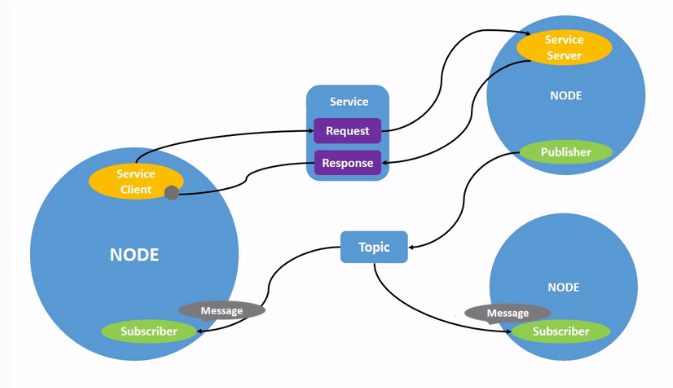
\includegraphics[width=\linewidth]{graph.png}
\caption{Graphical representation of Nodes using ROS \cite{RN202}}
\end{figure}

The official ROS documentation refers to Nodes as having a “modular purpose” \cite{RN202} and being capable of sending/receiving data from other nodes via Topics and Service. These Nodes are developed in C++ or Python. It is easy to get lost in all the specifics of ROS, luckily the developers do have tutorials and other documentation on the tool itself for individuals to get started(plus ROS is open source meaning there are alternatives even if the documentation is not useful \cite{RN200}). With the assistance of ROS implementing control/deploying the rovers will be simplified to focus on other aspects of the project. 
Although using ROS enables easier deployment of the tools needed for the project, simulations are an integral part of ensuring that the rovers operate as intended. To create simulations of the swarm, Gazebo will address this issue. Gazebo is 3D simulation software that integrates well with ROS\cite{RN202}. Like the ROS documentation Gazebo also offers some tutorials on getting started with it and how to operate it with ROS. Gazebo will allow us to test the rover code before programming and physically testing the rover themselves. This now leads to the question of how the rovers physically look and operate.

\subsubsection{Hardware}
For the hardware, let's first look at the brains of the rover, the development board. For the project, the rovers will use either the ESP32-DevKitC-32E and or ESP32-DevKitC-32UE by Espressif (the difference between the two is 32E uses a PCB antenna and 32UE uses an IPEX antenna \cite{RN203}). To list some of the specs of the device it has 448 KB ROM, 520 KB SRAM, it has WiFi, Bluetooth, UART, SPI, I2C, GPIO, ADC, and a lot of other features \cite{RN203}. However, this is all trivial when other boards also offer these features. Ultimately, the reason we are going to use the ESP32 is due to ROS being used to develop the rovers. ROS does not work with any microcontroller and needs specific ones to be able to operate. Essentially, these boards take advantage of “FreeRTOS, one of the three RTOSes officially supported by the micro-ROS project, which is natively used by this family of boards, and supports the latest Foxy release of ROS 2” \cite{RN204} and this does work with ROS 2 Humble version as well \cite{RN205}. For what is needed for the project these boards are perfect and will allow us to control the swarm of rovers via WiFi. There is also a chance that the project will also deploy a Raspberry PI 3 or 4 to be the central server, but given that at the time of writing, there is a supply chain issue with them, the central server will run on our machines/laptops. Now let us look at the rest of the body of the rover.
One of the challenges of getting the rover to work well together is to ensure that the rovers move predictably and accurately. To get the rovers to move there are a couple of items that are needed to do this correctly. The motors that are going to be used are simple DC Electric TT gear motors, these are cheap motors that are generally used in Arduino projects. However, the issue with these motors is that they do not have any form of encoding/giving feedback for knowing motor speed. To solve the problem of a lack of feedback, use of IR infrared slotted optical optocoupler module photo interrupter sensor, these are rotary encoders that can be attached to the motors for information on the motor speed and direction. Finally, with our custom H-bridge motor driver, we can use a PWM from the ESP32 to control the speed and direction of the motors. The three of these combined will allow us to accurately control and move the rovers despite the difference between motors. Then with the integration of a 2D lidar sensor, the rover will have the ability to perceive the world around them and avoid obstacles and other rovers. All of this, including the micro-controller, is being powered through a Lipo battery that can provide enough current and power to the system. Here is a wiring schematic of the rovers.

\begin{figure}
	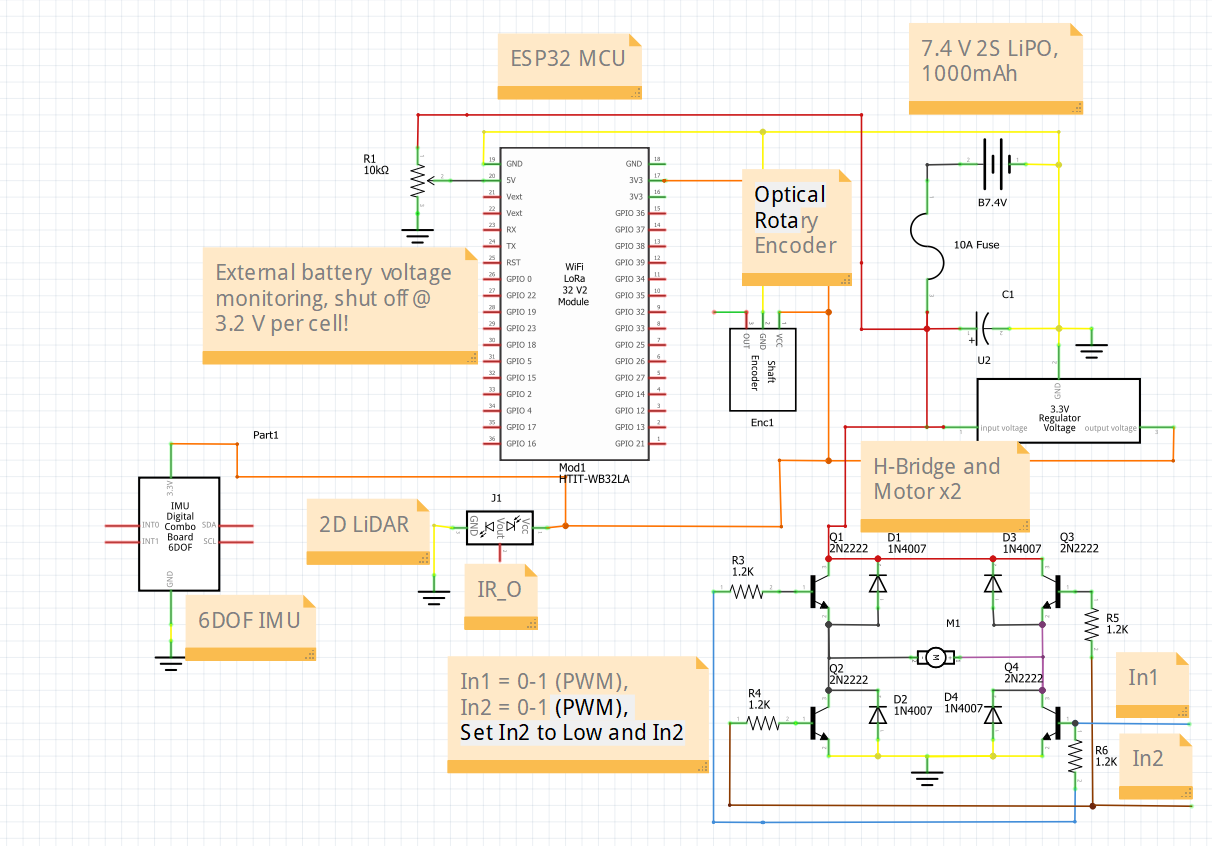
\includegraphics[width=\linewidth]{RoverWiringSchematic.png}
	\caption{Current Proposed wiring diagram of Rover}
\end{figure}

\section{Discussion}
Testing will be done regularly from the first-day our components arrive to assure quality and functionality. As we assemble each component together, testing will help in debugging and localizing the issue in the system. Creating tests for each component helps with creating a good understanding on how that device individually works as well as how it interacts with other devices and software. On the topic of software, testing is of critical importance, without testing the software integration could lead to unforeseen behavior within the system as a whole. If our tests were done correctly, on demo day it will present our flawless creation, the freedom rover units to the world.
\section{Demo Description} 
Our goal is to demonstrate one of these three demos on demo day. The First demo shows each drone/rover coordinating with one another to align themself to make a letter. An example of this demo: from the server we give the task of creating the letter ‘L’, with 5 drones scattered on the map, each rover will represent a pixel and will move to that spot. If there were two rovers that are the same distance away from a spot, one rover will have higher priority over the other and the rover with the higher priority will get that spot. As for the other rover it will go to the next closest open spot. Another option for the First demo, is that each rover will have multiple different LED lights to make a light show on the ground.

The Second demo is to have the rovers coordinate with one another to move an object from one location to another. An example: 3 rovers scattered around the map. The map is 5’ by 5’, where (0,0) is located at the bottom left corner and (5,5) is located at the top right corner. Each rover get the task to move a cardboard box from (1,1) to (4,3). All 3 rovers will communicate and align themselves around the box, to move it to the said location. Once done, they will wait for their next instruction which may be to move it to a different location. 

As for our last demo, the Third demo shows drones moving in a line around the map. For example: there are 2 tasks, the first task is to follow behind another drone and the second task is to move around the map. The second task will be given to one rover only and the first task will be given to all the other drones on the map. In this demo, there are 5 drones scattered throughout map and drone named \#2 will get the second task. As for the other Drones: \#1,\#3,\#4,\#5, they will get the first task. Let’s say the order of drone conga line is : \#2,\#3,\#1,\#5,\#4. If we were to separate \#1 from the conga line and place it elsewhere on the map, it will find its way behind the last rover in the congo line which in this case is \#4. Thus conga line will look like: \#2,\#3,\#5,\#4,\#1.

\section{Mitigation and Risks}
As with any project, there are challenges and risks that need to be addressed as the project progresses. The first is the issue of what happens when one breaks or gets to us broken. To solve this issue spare parts will be ordered as a precaution when the team has more money available. Parts are going to be tested to ensure they are working properly and safe handling of said parts to avoid accidental breaking. The simulation aspect of the rover brings with it a unique set of risks, if the teams spend too much time in simulation, unforeseen issues may occur when trying to translate/test in bulk with the physical rovers. To avoid this, incremental testing will be done to ensure that each step of the process is working. Time is also a big risk, with a project as large as this one, the team plans on meeting and working over the summer to ensure that the project will be finished in time. Finally, there is the issue of the custom H-bridge and power circuit PCB. If those fail and cannot find the issue with them we may resort to premade circuit board vendors from places like Adafruit and Digikey. Overall, the biggest issue/risk of the project is taking good care of the parts and ensuring they work because devices such as the 2D Lidar and Lipo batteries are expensive. We would rather not have to buy more than what we need.

\nocite{*}
\bibliographystyle{ieeetran}
\bibliography{InitialProposalDocBib}% Produces the bibliography via BibTeX.
\vspace{12pt}

\end{document}
